\phantomsection
\section*{BUỔI 2: CẤU HÌNH MONGODB}
\addcontentsline{toc}{section}{\numberline{}Buổi 2: Cấu hình MongoDB}
\setcounter{section}{2}
% =========================================================
% \clearpage
\phantomsection
\subsection*{Bước 0: Cài đặt MongoDB}
\addcontentsline{toc}{subsection}{\numberline{}Bước 0: Cài đặt MongoDB}
\setcounter{subsection}{1}
\setcounter{figure}{0}
\begin{figure}[H]
  \centering
  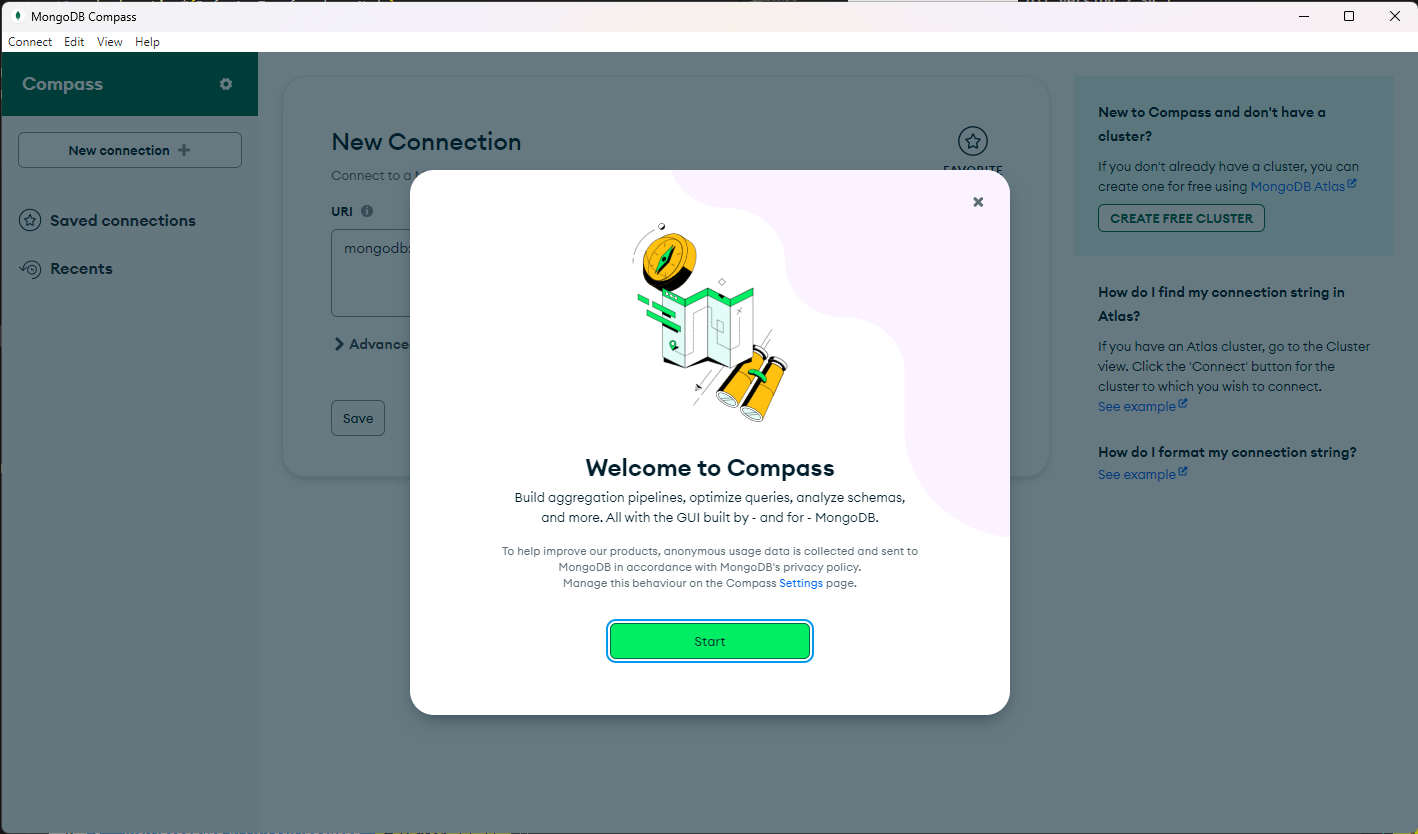
\includegraphics[width=15cm]{images/chapterSecond/1.png}
  \caption{\bfseries Cài đặt xong MongoDB Community Server}
\end{figure}
% =========================================================
\phantomsection
\subsection*{Bước 1: Cài đặt thư viện mongodb, định nghĩa hàm trợ giúp kết nối và lớp dịch vụ truy xuất cơ sở dữ liệu (CSDL)}
\addcontentsline{toc}{subsection}{\numberline{}Bước 1: Cài đặt thư viện mongodb, định nghĩa hàm trợ giúp kết nối và lớp dịch vụ truy xuất cơ sở dữ liệu (CSDL)}
\setcounter{subsection}{2}
\setcounter{figure}{0}
\begin{figure}[H]
  \centering
  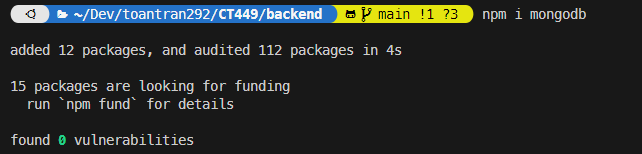
\includegraphics[width=15cm]{images/chapterSecond/2.png}
  \caption{\bfseries Cài đặt mongodb trong node}
\end{figure}
\begin{figure}[H]
  \centering
  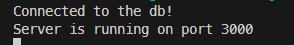
\includegraphics{images/chapterSecond/3.png}
  \caption{\bfseries Connect thành công tới database}
\end{figure}
% =========================================================
\phantomsection
\subsection*{Bước 2: Cài đặt các handler}
\addcontentsline{toc}{subsection}{\numberline{}Bước 2: Cài đặt các handler}
\setcounter{subsection}{3}
\setcounter{figure}{0}

\phantomsection
\subsubsection*{Cài đặt handler create}
\addcontentsline{toc}{subsubsection}{\numberline{}Cài đặt handler create}
\begin{figure}[H]
  \centering
  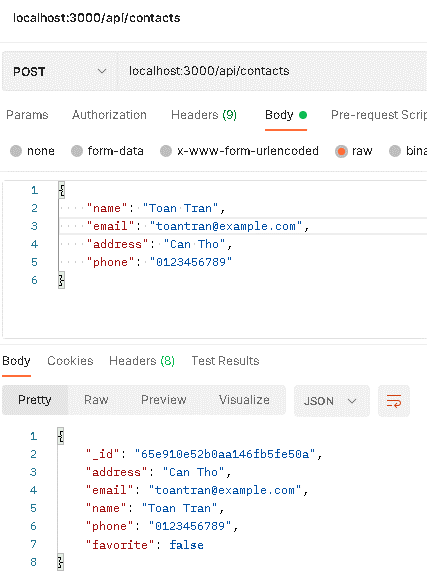
\includegraphics{images/chapterSecond/4.png}
  \caption{\bfseries Test API create bằng Postman}
\end{figure}
\phantomsection
\subsubsection*{Cài đặt handler findAll}
\addcontentsline{toc}{subsubsection}{\numberline{}Cài đặt handler findAll}
\begin{figure}[H]
  \centering
  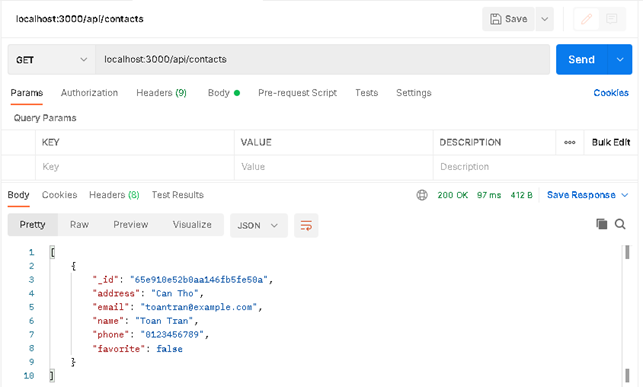
\includegraphics[width=15cm]{images/chapterSecond/5.png}
  \caption{\bfseries Test API get all bằng Postman}
\end{figure}
\begin{figure}[H]
  \centering
  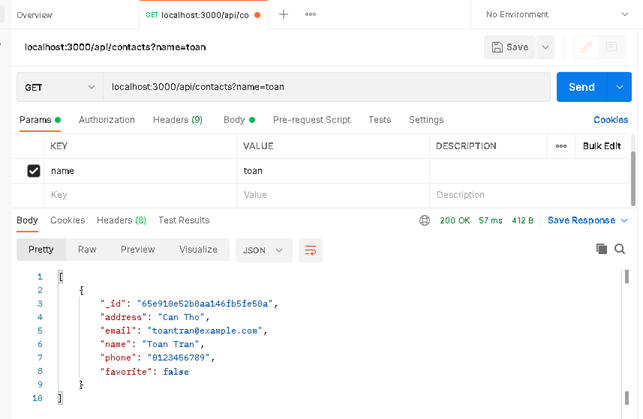
\includegraphics[width=15cm]{images/chapterSecond/6.png}
  \caption{\bfseries Test API get all kèm filter bằng Postman}
\end{figure}
\phantomsection
\subsubsection*{Cài đặt handler findOne}
\addcontentsline{toc}{subsubsection}{\numberline{}Cài đặt handler findOne}
\begin{figure}[H]
  \centering
  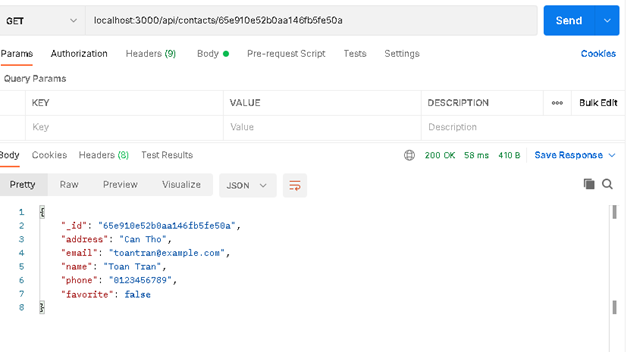
\includegraphics[width=15cm]{images/chapterSecond/7.png}
  \caption{\bfseries Test API get one bằng Postman}
\end{figure}
\phantomsection
\subsubsection*{Cài đặt handler update}
\addcontentsline{toc}{subsubsection}{\numberline{}Cài đặt handler update}
\begin{figure}[H]
  \centering
  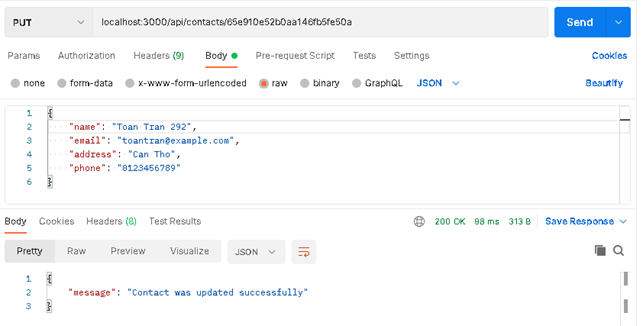
\includegraphics[width=15cm]{images/chapterSecond/8.png}
  \caption{\bfseries Test API update bằng Postman}
\end{figure}
\phantomsection
\subsubsection*{Cài đặt handler delete}
\addcontentsline{toc}{subsubsection}{\numberline{}Cài đặt handler delete}
\begin{figure}[H]
  \centering
  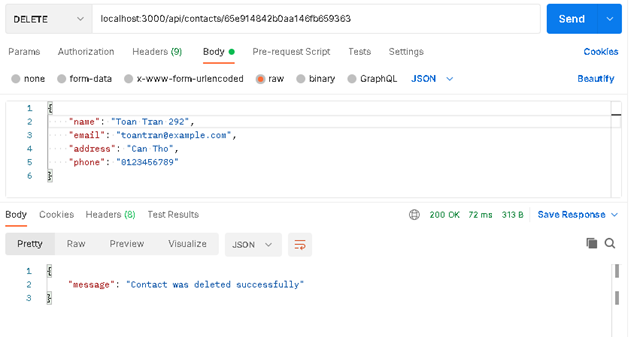
\includegraphics[width=15cm]{images/chapterSecond/9.png}
  \caption{\bfseries Test API delete bằng Postman}
\end{figure}
\phantomsection
\subsubsection*{Cài đặt handler findAllFavorite}
\addcontentsline{toc}{subsubsection}{\numberline{}Cài đặt handler findAllFavorite}
\begin{figure}[H]
  \centering
  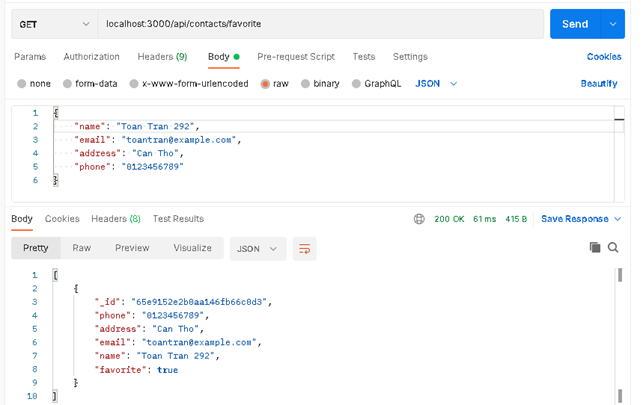
\includegraphics[width=15cm]{images/chapterSecond/10.png}
  \caption{\bfseries Test API get all favorites bằng Postman}
\end{figure}
\phantomsection
\subsubsection*{Cài đặt handler deleteAll}
\addcontentsline{toc}{subsubsection}{\numberline{}Cài đặt handler deleteAll}
\begin{figure}[H]
  \centering
  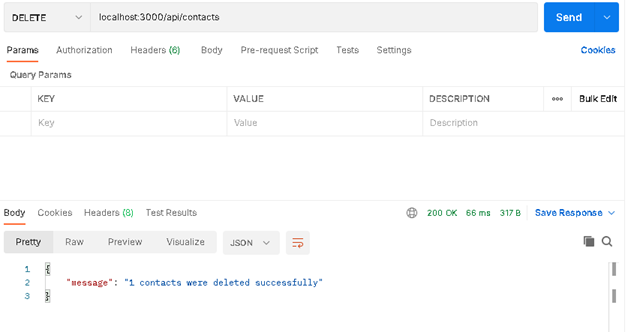
\includegraphics[width=15cm]{images/chapterSecond/11.png}
  \caption{\bfseries Test API delete all bằng Postman}
\end{figure}



% =========================================================
